\section{Radionuclide Transport Base Cases}\label{sec:nuclide_base_cases}
\subsection{No Release Problem Specification}
The no release base cases tested basic null containment transport behavior of 
all the radionuclide transport models at each component interface. This test 
neglected thermal transport and capacity estimation to simplify validation. 

The problem design includes : 
\begin{itemize}
\item{A source facility providing one waste stream per timestep}
\item{A legislated repository capacity of 5 1kg waste streams}
\item{A waste form Component} 
\item{A waste package Component}
\item{A buffer Component}
\item{A far field Component}
\end{itemize}

\subsubsection{Degradation Rate Model}
The Degradation Rate model should not release contaminants if the degradation 
rate is 0. Thus, four simulations were run to demonstrate total containment 
behavior at the Waste Form, Waste Package, Buffer, and Far Field interfaces 
respectively. 

\input{./chapters/demonstration/no_release/dr_no_release_tab}

\begin{figure}[ht]
\centering
\includegraphics[width=0.8\textwidth]{./chapters/demonstration/no_release/wf0deg.eps}
\caption[$^{235}U$ residence. Degradation Rate Waste Form No Release.]{
For Case DRI, in which total containment in the waste form is assumed ($F_{d,wf}=0$), 
$^{235}U$ takes up permanent residence in the buffer component.
}
\label{fig:drIall}
\begin{minipage}[b]{0.45\linewidth}

  \includegraphics[width=\textwidth]{./chapters/demonstration/no_release/wf0deg1.eps}
  \caption[DRI Waste Form Contaminants.]{
    Waste Form 5 ($F_d = 0$) never releases material.
    }
  \label{fig:drIwf5}
  
  \includegraphics[width=\textwidth]{./chapters/demonstration/no_release/wf0deg3.eps}
  \caption[Case DRI Buffer Contaminants]{
    The Buffer, component 7 ($F_d = 0.1$), never recieves material.
    }
  \label{fig:drIbuff}

\end{minipage}
\hspace{0.05\linewidth}
\begin{minipage}[b]{0.45\linewidth}
  \includegraphics[width=\textwidth]{./chapters/demonstration/no_release/wf0deg2.eps}
  \caption[Case DRI Waste Package Contaminants.]{ 
    Waste Package 6 ($F_d = 0.1$), never recieves material.
    }
  \label{fig:drIwp6}

  \includegraphics[width=\textwidth]{./chapters/demonstration/no_release/wf0deg0.eps}
  \caption[Case DRI Far Field Contaminants.]{ 
    The Far Field, component 0 ($F_d = 0.1$), never recieves material.
    }
  \label{fig:drIff0}

  \end{minipage}
\end{figure}
\clearpage



\begin{figure}[ht]
\centering
\includegraphics[width=0.8\textwidth]{./chapters/demonstration/no_release/wp0deg.eps}
\caption[$^{235}U$ residence. Degradation Rate Waste Package No Release.]{
For Case DRII, in which total containment in the waste package is assumed ($F_{d,wp}=0$), 
$^{235}U$ travels through waste forms ($F_d = 0.1$) before 
permanent residence in the waste package components.
}
\label{fig:drIIall}
\begin{minipage}[b]{0.45\linewidth}

  \includegraphics[width=\textwidth]{./chapters/demonstration/no_release/wp0deg1.eps}
  \caption[DRII Waste Form Contaminants.]{
    Waste Form 5 ($F_d = 0.1$) releases material with degradation. 
    }
  \label{fig:drIIwf5}
  
  \includegraphics[width=\textwidth]{./chapters/demonstration/no_release/wp0deg3.eps}
  \caption[Case DRII Buffer Contaminants]{
    The Buffer, component 7 ($F_d = 0.1$), never recieves material.
    }
  \label{fig:drIIbuff}

\end{minipage}
\hspace{0.05\linewidth}
\begin{minipage}[b]{0.45\linewidth}
  \includegraphics[width=\textwidth]{./chapters/demonstration/no_release/wp0deg2.eps}
  \caption[Case DRII Waste Package Contaminants.]{ 
    Waste Package 6 ($F_d = 0$) acheives total containment.
    }
  \label{fig:drIIwp6}

  \includegraphics[width=\textwidth]{./chapters/demonstration/no_release/wp0deg0.eps}
  \caption[Case DRII Far Field Contaminants.]{ 
    The Far Field, component 0 ($F_d = 0.1$), never recieves material.
    }
  \label{fig:drIIff0}


  \end{minipage}
\end{figure}
\clearpage

\begin{figure}[ht]
\centering
\includegraphics[width=0.8\textwidth]{./chapters/demonstration/no_release/buff0deg.eps}
\caption[$^{235}U$ residence. Degradation Rate Buffer No Release.]{
For Case DRIII, in which total containment in the buffer is assumed ($F_{d,buffer}=0$), 
$^{235}U$ travels through waste forms and waste package components ($F_d = 0.1$) before 
permanent residence in the buffer component.
}
\label{fig:drIIIall}
\begin{minipage}[b]{0.45\linewidth}

  \includegraphics[width=\textwidth]{./chapters/demonstration/no_release/buff0deg1.eps}
  \caption[DRIII Waste Form Contaminants.]{
    Waste Form 5 ($F_d = 0.1$) releases material with degradation. 
    }
  \label{fig:drIIIwf5}
  
  \includegraphics[width=\textwidth]{./chapters/demonstration/no_release/buff0deg3.eps}
  \caption[Case DRIII Buffer Contaminants]{
    The Buffer, component 7 ($F_d=0$), acheives total containment.
    }
  \label{fig:drIIIbuff}

\end{minipage}
\hspace{0.05\linewidth}
\begin{minipage}[b]{0.45\linewidth}
  \includegraphics[width=\textwidth]{./chapters/demonstration/no_release/buff0deg2.eps}
  \caption[Case DRIII Waste Package Contaminants.]{ 
    Waste Package 6 ($F_d = 0.1$) recieves then releases material. 
    }
  \label{fig:drIIIwp6}

  \includegraphics[width=\textwidth]{./chapters/demonstration/no_release/buff0deg0.eps}
  \caption[Case DRIII Waste Package Contaminants.]{ 
    The Far Field, component 0 ($F_d = 0.1$), never recieves material.
    }
  \label{fig:drIIIff0}


  \end{minipage}
\end{figure}
\clearpage



\begin{figure}[ht]
\centering
\includegraphics[width=0.8\textwidth]{./chapters/demonstration/no_release/buff0deg.eps}
\caption[$^{235}U$ residence. Degradation Rate Buffer No Release.]{
For DRIII case in which total containment in the buffer is assumed ($F_{d,buffer}=0$), 
$^{235}U$ travels through waste forms and waste package components ($F_d = 0.1$) before 
permanent residence in the buffer component.
}
\label{fig:drIIIall}
\begin{minipage}[b]{0.45\linewidth}

  \includegraphics[width=\textwidth]{./chapters/demonstration/no_release/buff0deg1.eps}
  \caption[DRIII Waste Form Contaminants.]{
    Waste Form 5 ($F_d = 0.1$) releases material with degradation. 
    }
  \label{fig:drIIIwf5}
  
  \includegraphics[width=\textwidth]{./chapters/demonstration/no_release/buff0deg3.eps}
  \caption[Case DRIII Buffer Contaminants]{
    The Buffer, component 7 ($F_d=0$), acheives total containment.
    }
  \label{fig:drIIIbuff}

\end{minipage}
\hspace{0.05\linewidth}
\begin{minipage}[b]{0.45\linewidth}
  \includegraphics[width=\textwidth]{./chapters/demonstration/no_release/buff0deg2.eps}
  \caption[Case DRIII Waste Package Contaminants.]{ 
    Waste Package 6 ($F_d = 0.1$) recieves then releases material. 
    }
  \label{fig:drIIIwp6}

  \includegraphics[width=\textwidth]{./chapters/demonstration/no_release/buff0deg0.eps}
  \caption[Case DRIII Waste Package Contaminants.]{ 
    The Far Field, component 0 ($F_d = 0.1$), never recieves material.
    }
  \label{fig:drIIIff0}


  \end{minipage}
\end{figure}

\clearpage

\subsubsection{Mixed Cell Model}

\begin{table}
\centering
\begin{tabular}{|l|c|c|r|}
  \hline
  \multicolumn{4}{c}{\textbf{Mixed Cell Model No Release Contaminant Transport}}\\
  \hline
  \textbf{Case}  &  \textbf{Component} &  \textbf{Degradation Rate} & \textbf{Expected 10 yrs} & \textbf{Actual 10 yrs}\\
  \textbf{ID}    & \textbf{[Type]} &  \textbf{$[yr^{-1}]$}  &  $[\%]$  & $[\%]$\\
  \hline
  MCI     &  WF    &  0   & 1\\
          &  WP    &  0.1 & 0\\
          &  BUFF  &  0.1 & 0\\
          &  FF    &  0.1 & 0\\
  \hline
  MCII    &  WF    &  0.1 & 0\\
          &  WP    &  0   & 1\\
          &  BUFF  &  0.1 & 0\\
          &  FF    &  0.1 & 0\\
  \hline
  MCIII   &  WF    &  0.1 & 0\\
          &  WP    &  0.1 & 0\\
          &  BUFF  &  0   & 1\\
          &  FF    &  0.1 & 0\\
  \hline
  MCIV    &  WF    &  0.1 & 0\\
          &  WP    &  0.1 & 0\\
          &  BUFF  &  0.1 & 0\\
          &  FF    &  0   & 1\\
  \hline
\end{tabular}
\caption{<+Caption text+>}
\label{tab:<+label+>}
\end{table}<++>

\begin{figure}[ht]
\begin{minipage}[b]{0.45\linewidth}
\centering
\includegraphics[width=\textwidth]{./chapters/demonstration/no_release/buff0deg.eps}
\includegraphics[width=\textwidth]{./chapters/demonstration/no_release/buff0deg1.eps}
\caption{default}
\label{fig:figure1}
\end{minipage}
\hspace{0.5cm}
\begin{minipage}[b]{0.45\linewidth}
\centering
\includegraphics[width=\textwidth]{./chapters/demonstration/no_release/buff0deg2.eps}
\includegraphics[width=\textwidth]{./chapters/demonstration/no_release/buff0deg3.eps}
\caption{default}
\label{fig:figure2}
\end{minipage}
\end{figure}

\clearpage

\subsubsection{Lumped Parameter Model}

\input{./chapters/demonstration/no_release/lp_no_release_tab}




\begin{figure}[ht]
\centering
\includegraphics[width=0.8\textwidth]{./chapters/demonstration/no_release/lpEMI.eps}
\caption[$^{235}U$ residence. Lumped Parameter EM Waste Form No Release.]{
For case LPEMI in which total containment in the waste form is assumed 
($F_{d,wf}=0$), $^{235}U$ 
takes permanent residence in the waste form component.
}
\label{fig:lpEMIall}
\begin{minipage}[b]{0.45\linewidth}

  \includegraphics[width=\textwidth]{./chapters/demonstration/no_release/lpEMI1.eps}
  \caption[LPEMI Waste Form Contaminants.]{
    Waste Form 5 ($F_d = 0.1$) releases material with degradation. 
    }
  \label{fig:lpEMIwf5}
  
  \includegraphics[width=\textwidth]{./chapters/demonstration/no_release/lpEMI3.eps}
  \caption[Case LPEMI Buffer Contaminants]{
    The Buffer, component 7 ($F_d=0$), acheives total containment.
    }
  \label{fig:lpEMIbuff}

\end{minipage}
\hspace{0.05\linewidth}
\begin{minipage}[b]{0.45\linewidth}
  \includegraphics[width=\textwidth]{./chapters/demonstration/no_release/lpEMI2.eps}
  \caption[Case LPEMI Waste Package Contaminants.]{ 
    Waste Package 6 ($F_d = 0.1$) recieves then releases material. 
    }
  \label{fig:lpEMIwp6}

  \includegraphics[width=\textwidth]{./chapters/demonstration/no_release/lpEMI0.eps}
  \caption[Case LPEMI Waste Package Contaminants.]{ 
    The Far Field, component 0 ($F_d = 0.1$), never recieves material.
    }
  \label{fig:lpEMIff0}


  \end{minipage}
\end{figure}
\begin{figure}[ht]
\centering
\includegraphics[width=0.8\textwidth]{./chapters/demonstration/no_release/lpEMII.eps}
\caption[$^{235}U$ residence. Lumped Parameter  Waste Package No Release.]{
For case LPEMII in which total containment in the waste package is assumed 
($F_{d,wp}=0$), $^{235}U$ travels through the waste form component ($F_d = 0.1$) before 
permanent residence in the waste package component.
}
\label{fig:lpEMIIall}
\begin{minipage}[b]{0.45\linewidth}

  \includegraphics[width=\textwidth]{./chapters/demonstration/no_release/lpEMII1.eps}
  \caption[LPEMII Waste Form Contaminants.]{
    Waste Form 5 ($F_d = 0.1$) releases material with degradation. 
    }
  \label{fig:lpEMIIwf5}
  
  \includegraphics[width=\textwidth]{./chapters/demonstration/no_release/lpEMII3.eps}
  \caption[Case LPEMII Buffer Contaminants]{
    The Buffer, component 7 ($F_d=0$), acheives total containment.
    }
  \label{fig:lpEMIIbuff}

\end{minipage}
\hspace{0.05\linewidth}
\begin{minipage}[b]{0.45\linewidth}
  \includegraphics[width=\textwidth]{./chapters/demonstration/no_release/lpEMII2.eps}
  \caption[Case LPEMII Waste Package Contaminants.]{ 
    Waste Package 6 ($F_d = 0.1$) recieves then releases material. 
    }
  \label{fig:lpEMIIwp6}

  \includegraphics[width=\textwidth]{./chapters/demonstration/no_release/lpEMII0.eps}
  \caption[Case LPEMII Waste Package Contaminants.]{ 
    The Far Field, component 0 ($F_d = 0.1$), never recieves material.
    }
  \label{fig:lpEMIIff0}


  \end{minipage}
\end{figure}
%\begin{figure}[ht]
%\centering
%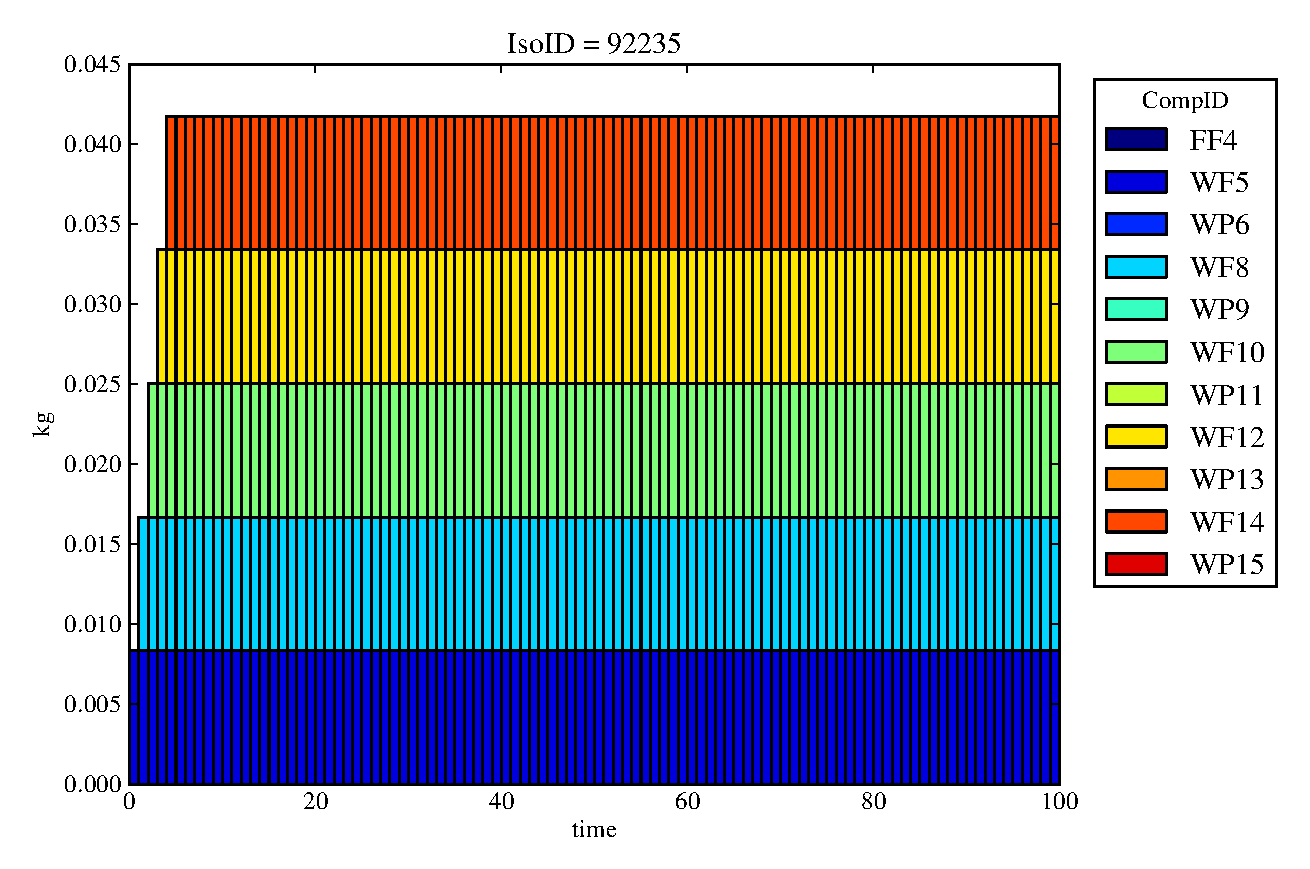
\includegraphics[width=0.8\textwidth]{./chapters/demonstration/no_release/lpEMIII.eps}
%\caption[$^{235}U$ residence. Lumped Parameter  <+Component+> No Release.]{
%For <+CASE+> case in which total containment in the <+component+> is assumed 
%($F_{d,<+comp+>}=0$), $^{235}U$ travels through  components ($F_d = 0.1$) before 
%permanent residence in the <+component+> component.
%}
%\label{fig:lpEMIIIall}
%\begin{minipage}[b]{0.45\linewidth}
%
%  \includegraphics[width=\textwidth]{./chapters/demonstration/no_release/lpEMIII1.eps}
%  \caption[LPEMIII Waste Form Contaminants.]{
%    Waste Form 5 ($F_d = 0.1$) releases material with degradation. 
%    }
%  \label{fig:lpEMIIIwf5}
%  
%  \includegraphics[width=\textwidth]{./chapters/demonstration/no_release/lpEMIII3.eps}
%  \caption[Case LPEMIII Buffer Contaminants]{
%    The Buffer, component 7 ($F_d=0$), acheives total containment.
%    }
%  \label{fig:lpEMIIIbuff}
%
%\end{minipage}
%\hspace{0.05\linewidth}
%\begin{minipage}[b]{0.45\linewidth}
%  \includegraphics[width=\textwidth]{./chapters/demonstration/no_release/lpEMIII2.eps}
%  \caption[Case LPEMIII Waste Package Contaminants.]{ 
%    Waste Package 6 ($F_d = 0.1$) recieves then releases material. 
%    }
%  \label{fig:lpEMIIIwp6}
%
%  \includegraphics[width=\textwidth]{./chapters/demonstration/no_release/lpEMIII0.eps}
%  \caption[Case LPEMIII Waste Package Contaminants.]{ 
%    The Far Field, component 0 ($F_d = 0.1$), never recieves material.
%    }
%  \label{fig:lpEMIIIff0}
%
%
%  \end{minipage}
%\end{figure}
%\begin{figure}[ht]
%\centering
%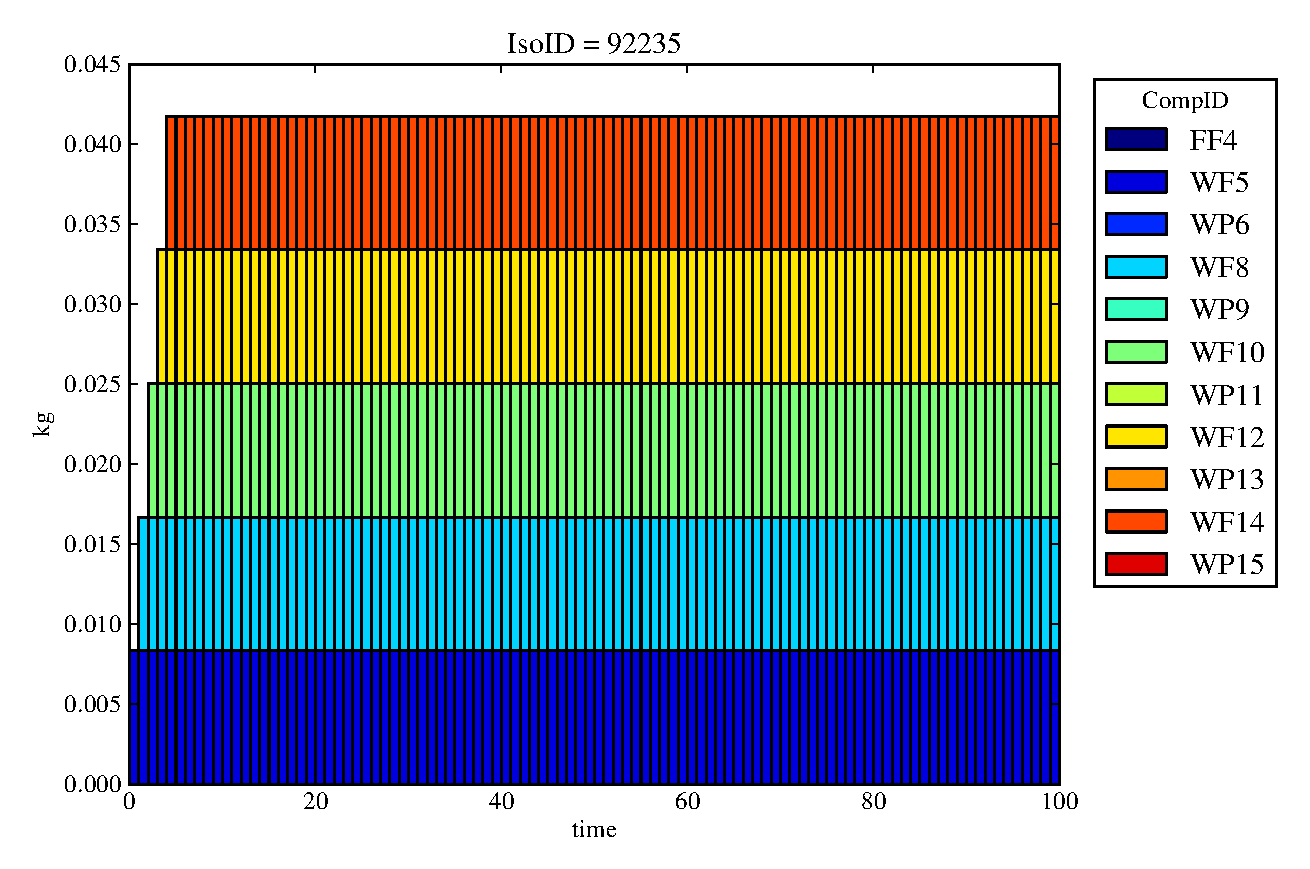
\includegraphics[width=0.8\textwidth]{./chapters/demonstration/no_release/lpEMIV.eps}
%\caption[$^{235}U$ residence. Lumped Parameter  <+Component+> No Release.]{
%For <+CASE+> case in which total containment in the <+component+> is assumed 
%($F_{d,<+comp+>}=0$), $^{235}U$ travels through  components ($F_d = 0.1$) before 
%permanent residence in the <+component+> component.
%}
%\label{fig:lpEMIVall}
%\begin{minipage}[b]{0.45\linewidth}
%
%  \includegraphics[width=\textwidth]{./chapters/demonstration/no_release/lpEMIV1.eps}
%  \caption[LPEMIV Waste Form Contaminants.]{
%    Waste Form 5 ($F_d = 0.1$) releases material with degradation. 
%    }
%  \label{fig:lpEMIVwf5}
%  
%  \includegraphics[width=\textwidth]{./chapters/demonstration/no_release/lpEMIV3.eps}
%  \caption[Case LPEMIV Buffer Contaminants]{
%    The Buffer, component 7 ($F_d=0$), acheives total containment.
%    }
%  \label{fig:lpEMIVbuff}
%
%\end{minipage}
%\hspace{0.05\linewidth}
%\begin{minipage}[b]{0.45\linewidth}
%  \includegraphics[width=\textwidth]{./chapters/demonstration/no_release/lpEMIV2.eps}
%  \caption[Case LPEMIV Waste Package Contaminants.]{ 
%    Waste Package 6 ($F_d = 0.1$) recieves then releases material. 
%    }
%  \label{fig:lpEMIVwp6}
%
%  \includegraphics[width=\textwidth]{./chapters/demonstration/no_release/lpEMIV0.eps}
%  caption[Case LPEMIV Waste Package Contaminants.]{ 
%    The Far Field, component 0 ($F_d = 0.1$), never recieves material.
%    }
%  \label{fig:lpEMIVff0}
%
%
%  \end{minipage}
%\end{figure}
\clearpage

%%%%%%%%%%%%%%%%%%%%%%%%%%%%%%
% DM
%%%%%%%%%%%%%%%%%%%%%%%%%%%%%%


\begin{figure}[ht]
\centering
\includegraphics[width=0.8\textwidth]{./chapters/demonstration/no_release/lpDMI.eps}
\caption[$^{235}U$ residence. Lumped Parameter  DM Waste Form No Release.]{
For case LPDMI  in which total containment in the waste form is assumed 
($F_{d,wf}=0$), $^{235}U$ 
takes permanent residence in the waste form  component.
}
\label{fig:lpDMIall}
\begin{minipage}[b]{0.45\linewidth}

  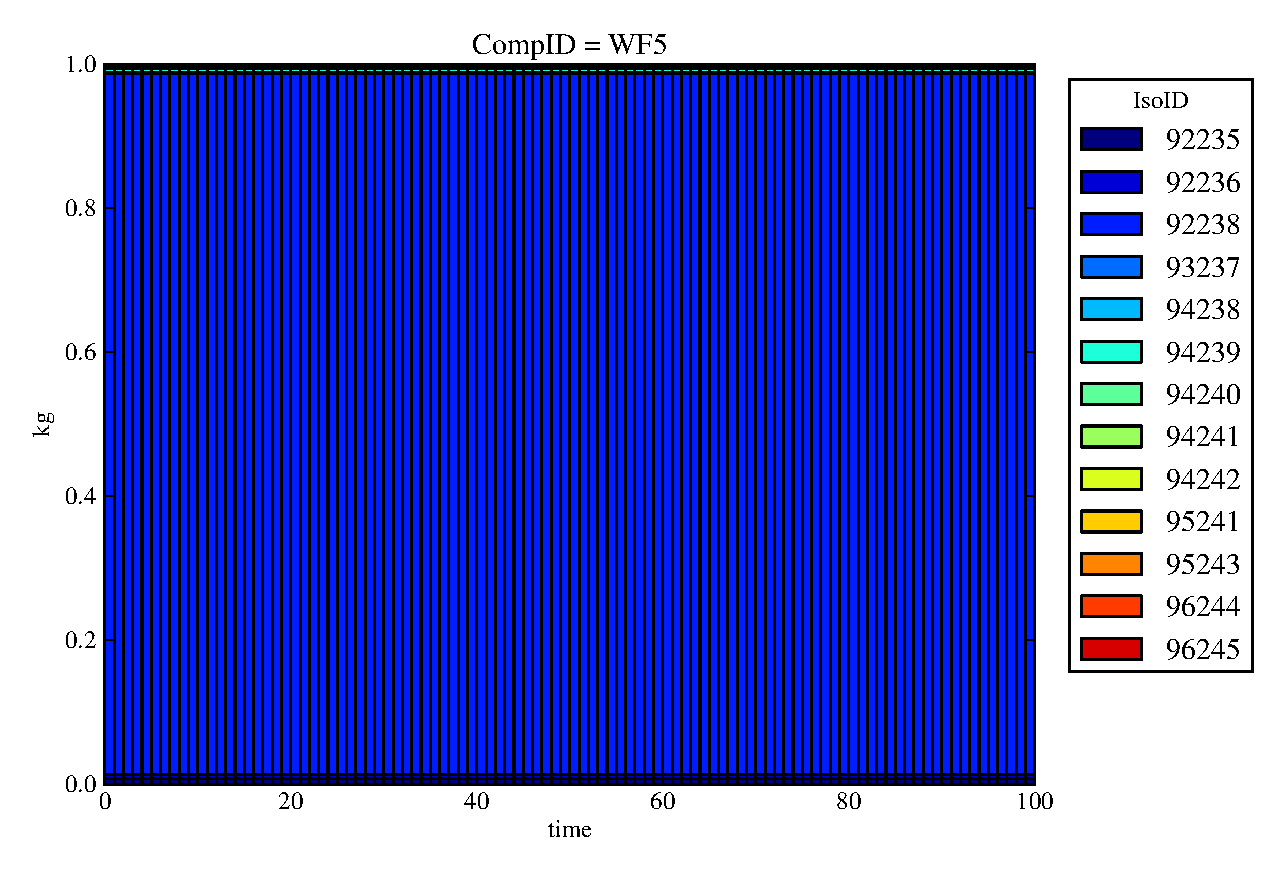
\includegraphics[width=\textwidth]{./chapters/demonstration/no_release/lpDMI1.eps}
  \caption[LPDMI Waste Form Contaminants.]{
    Waste Form 5 ($F_d = 0.1$) releases material with degradation. 
    }
  \label{fig:lpDMIwf5}
  
  \includegraphics[width=\textwidth]{./chapters/demonstration/no_release/lpDMI3.eps}
  \caption[Case LPDMI Buffer Contaminants]{
    The Buffer, component 7 ($F_d=0$), acheives total containment.
    }
  \label{fig:lpDMIbuff}

\end{minipage}
\hspace{0.05\linewidth}
\begin{minipage}[b]{0.45\linewidth}
  \includegraphics[width=\textwidth]{./chapters/demonstration/no_release/lpDMI2.eps}
  \caption[Case LPDMI Waste Package Contaminants.]{ 
    Waste Package 6 ($F_d = 0.1$) recieves then releases material. 
    }
  \label{fig:lpDMIwp6}

  \includegraphics[width=\textwidth]{./chapters/demonstration/no_release/lpDMI0.eps}
  \caption[Case LPDMI Waste Package Contaminants.]{ 
    The Far Field, component 0 ($F_d = 0.1$), never recieves material.
    }
  \label{fig:lpDMIff0}


  \end{minipage}
\end{figure}
\begin{figure}[ht]
\centering
\includegraphics[width=0.8\textwidth]{./chapters/demonstration/no_release/lpDMII.eps}
\caption[$^{235}U$ residence. Lumped Parameter  DM Waste Package No Release.]{
For LPDMII case in which total containment in the waste package is assumed 
($F_{d,wp}=0$), $^{235}U$ travels through the waste form component ($F_d = 0.1$) before 
permanent residence in the waste form component.
}
\label{fig:lpDMIIall}
\begin{minipage}[b]{0.45\linewidth}

  \includegraphics[width=\textwidth]{./chapters/demonstration/no_release/lpDMII1.eps}
  \caption[LPDMII Waste Form Contaminants.]{
    Waste Form 5 ($F_d = 0.1$) releases material with degradation. 
    }
  \label{fig:lpDMIIwf5}
  
  \includegraphics[width=\textwidth]{./chapters/demonstration/no_release/lpDMII3.eps}
  \caption[Case LPDMII Buffer Contaminants]{
    The Buffer, component 7 ($F_d=0$), acheives total containment.
    }
  \label{fig:lpDMIIbuff}

\end{minipage}
\hspace{0.05\linewidth}
\begin{minipage}[b]{0.45\linewidth}
  \includegraphics[width=\textwidth]{./chapters/demonstration/no_release/lpDMII2.eps}
  \caption[Case LPDMII Waste Package Contaminants.]{ 
    Waste Package 6 ($F_d = 0.1$) recieves then releases material. 
    }
  \label{fig:lpDMIIwp6}

  \includegraphics[width=\textwidth]{./chapters/demonstration/no_release/lpDMII0.eps}
  \caption[Case LPDMII Waste Package Contaminants.]{ 
    The Far Field, component 0 ($F_d = 0.1$), never recieves material.
    }
  \label{fig:lpDMIIff0}


  \end{minipage}
\end{figure}
%\begin{figure}[ht]
%\centering
%\includegraphics[width=0.8\textwidth]{./chapters/demonstration/no_release/lpDMIII.eps}
%\caption[$^{235}U$ residence. Lumped Parameter  <+Component+> No Release.]{
%For <+CASE+> case in which total containment in the <+component+> is assumed 
%($F_{d,<+comp+>}=0$), $^{235}U$ travels through  components ($F_d = 0.1$) before 
%permanent residence in the <+component+> component.
%}
%\label{fig:lpDMIIIall}
%\begin{minipage}[b]{0.45\linewidth}
%
%  \includegraphics[width=\textwidth]{./chapters/demonstration/no_release/lpDMIII1.eps}
%  \caption[LPDMIII Waste Form Contaminants.]{
%    Waste Form 5 ($F_d = 0.1$) releases material with degradation. 
%    }
%  \label{fig:lpDMIIIwf5}
%  
%  \includegraphics[width=\textwidth]{./chapters/demonstration/no_release/lpDMIII3.eps}
%  \caption[Case LPDMIII Buffer Contaminants]{
%    The Buffer, component 7 ($F_d=0$), acheives total containment.
%    }
%  \label{fig:lpDMIIIbuff}
%
%\end{minipage}
%\hspace{0.05\linewidth}
%\begin{minipage}[b]{0.45\linewidth}
%  \includegraphics[width=\textwidth]{./chapters/demonstration/no_release/lpDMIII2.eps}
%  \caption[Case LPDMIII Waste Package Contaminants.]{ 
%    Waste Package 6 ($F_d = 0.1$) recieves then releases material. 
%    }
%  \label{fig:lpDMIIIwp6}
%
%  \includegraphics[width=\textwidth]{./chapters/demonstration/no_release/lpDMIII0.eps}
%  \caption[Case LPDMIII Waste Package Contaminants.]{ 
%    The Far Field, component 0 ($F_d = 0.1$), never recieves material.
%    }
%  \label{fig:lpDMIIIff0}
%
%
%  \end{minipage}
%\end{figure}
%\begin{figure}[ht]
%\centering
%\includegraphics[width=0.8\textwidth]{./chapters/demonstration/no_release/lpDMIV.eps}
%\caption[$^{235}U$ residence. Lumped Parameter  <+Component+> No Release.]{
%For <+CASE+> case in which total containment in the <+component+> is assumed 
%($F_{d,<+comp+>}=0$), $^{235}U$ travels through  components ($F_d = 0.1$) before 
%permanent residence in the <+component+> component.
%}
%\label{fig:lpDMIVall}
%\begin{minipage}[b]{0.45\linewidth}
%
%  \includegraphics[width=\textwidth]{./chapters/demonstration/no_release/lpDMIV1.eps}
%  \caption[LPDMIV Waste Form Contaminants.]{
%    Waste Form 5 ($F_d = 0.1$) releases material with degradation. 
%    }
%  \label{fig:lpDMIVwf5}
%  
%  \includegraphics[width=\textwidth]{./chapters/demonstration/no_release/lpDMIV3.eps}
%  \caption[Case LPDMIV Buffer Contaminants]{
%    The Buffer, component 7 ($F_d=0$), acheives total containment.
%    }
%  \label{fig:lpDMIVbuff}
%
%\end{minipage}
%\hspace{0.05\linewidth}
%\begin{minipage}[b]{0.45\linewidth}
%  \includegraphics[width=\textwidth]{./chapters/demonstration/no_release/lpDMIV2.eps}
%  \caption[Case LPDMIV Waste Package Contaminants.]{ 
%    Waste Package 6 ($F_d = 0.1$) recieves then releases material. 
%    }
%  \label{fig:lpDMIVwp6}
%
%  \includegraphics[width=\textwidth]{./chapters/demonstration/no_release/lpDMIV0.eps}
%  caption[Case LPDMIV Waste Package Contaminants.]{ 
%    The Far Field, component 0 ($F_d = 0.1$), never recieves material.
%    }
%  \label{fig:lpDMIVff0}
%
%
%  \end{minipage}
%\end{figure}
\clearpage
%%%%%%%%%%%%%%%%%%%%%%%%%%%%%%%
% PFM
%%%%%%%%%%%%%%%%%%%%%%%%%%%%%%%



\begin{figure}[ht]
\centering
\includegraphics[width=0.8\textwidth]{./chapters/demonstration/no_release/lpPFMI.eps}
\caption[$^{235}U$ residence. Lumped Parameter PFM Waste Form No Release.]{
For case LPPFMI  in which total containment in the waste form is assumed 
($F_{d,wf}=0$), $^{235}U$ resides permanently in the waste form component.
}
\label{fig:lpPFMIall}
\begin{minipage}[b]{0.45\linewidth}

  \includegraphics[width=\textwidth]{./chapters/demonstration/no_release/lpPFMI1.eps}
  \caption[LPPFMI Waste Form Contaminants.]{
    Waste Form 5 ($F_d = 0.1$) releases material with degradation. 
    }
  \label{fig:lpPFMIwf5}
  
  \includegraphics[width=\textwidth]{./chapters/demonstration/no_release/lpPFMI3.eps}
  \caption[Case LPPFMI Buffer Contaminants]{
    The Buffer, component 7 ($F_d=0$), acheives total containment.
    }
  \label{fig:lpPFMIbuff}

\end{minipage}
\hspace{0.05\linewidth}
\begin{minipage}[b]{0.45\linewidth}
  \includegraphics[width=\textwidth]{./chapters/demonstration/no_release/lpPFMI2.eps}
  \caption[Case LPPFMI Waste Package Contaminants.]{ 
    Waste Package 6 ($F_d = 0.1$) recieves then releases material. 
    }
  \label{fig:lpPFMIwp6}

  \includegraphics[width=\textwidth]{./chapters/demonstration/no_release/lpPFMI0.eps}
  \caption[Case LPPFMI Waste Package Contaminants.]{ 
    The Far Field, component 0 ($F_d = 0.1$), never recieves material.
    }
  \label{fig:lpPFMIff0}


  \end{minipage}
\end{figure}
\begin{figure}[ht]
\centering
\includegraphics[width=0.8\textwidth]{./chapters/demonstration/no_release/lpPFMII.eps}
\caption[$^{235}U$ residence. Lumped Parameter PFM Waste Package No Release.]{
For case LPPFMII in which total containment in the waste package is assumed 
($F_{d,wp}=0$), $^{235}U$ travels through the waste form component ($F_d = 0.1$) before 
permanent residence in the waste package component.
}
\label{fig:lpPFMIIall}
\begin{minipage}[b]{0.45\linewidth}

  \includegraphics[width=\textwidth]{./chapters/demonstration/no_release/lpPFMII1.eps}
  \caption[LPPFMII Waste Form Contaminants.]{
    Waste Form 5 ($F_d = 0.1$) releases material with degradation. 
    }
  \label{fig:lpPFMIIwf5}
  
  \includegraphics[width=\textwidth]{./chapters/demonstration/no_release/lpPFMII3.eps}
  \caption[Case LPPFMII Buffer Contaminants]{
    The Buffer, component 7 ($F_d=0$), acheives total containment.
    }
  \label{fig:lpPFMIIbuff}

\end{minipage}
\hspace{0.05\linewidth}
\begin{minipage}[b]{0.45\linewidth}
  \includegraphics[width=\textwidth]{./chapters/demonstration/no_release/lpPFMII2.eps}
  \caption[Case LPPFMII Waste Package Contaminants.]{ 
    Waste Package 6 ($F_d = 0.1$) recieves then releases material. 
    }
  \label{fig:lpPFMIIwp6}

  \includegraphics[width=\textwidth]{./chapters/demonstration/no_release/lpPFMII0.eps}
  \caption[Case LPPFMII Waste Package Contaminants.]{ 
    The Far Field, component 0 ($F_d = 0.1$), never recieves material.
    }
  \label{fig:lpPFMIIff0}


  \end{minipage}
\end{figure}
%\begin{figure}[ht]
%\centering
%\includegraphics[width=0.8\textwidth]{./chapters/demonstration/no_release/lpPFMIII.eps}
%\caption[$^{235}U$ residence. Lumped Parameter  <+Component+> No Release.]{
%For <+CASE+> case in which total containment in the <+component+> is assumed 
%($F_{d,<+comp+>}=0$), $^{235}U$ travels through  components ($F_d = 0.1$) before 
%permanent residence in the <+component+> component.
%}
%\label{fig:lpPFMIIIall}
%\begin{minipage}[b]{0.45\linewidth}
%
%  \includegraphics[width=\textwidth]{./chapters/demonstration/no_release/lpPFMIII1.eps}
%  \caption[LPPFMIII Waste Form Contaminants.]{
%    Waste Form 5 ($F_d = 0.1$) releases material with degradation. 
%    }
%  \label{fig:lpPFMIIIwf5}
%  
%  \includegraphics[width=\textwidth]{./chapters/demonstration/no_release/lpPFMIII3.eps}
%  \caption[Case LPPFMIII Buffer Contaminants]{
%    The Buffer, component 7 ($F_d=0$), acheives total containment.
%    }
%  \label{fig:lpPFMIIIbuff}
%
%\end{minipage}
%\hspace{0.05\linewidth}
%\begin{minipage}[b]{0.45\linewidth}
%  \includegraphics[width=\textwidth]{./chapters/demonstration/no_release/lpPFMIII2.eps}
%  \caption[Case LPPFMIII Waste Package Contaminants.]{ 
%    Waste Package 6 ($F_d = 0.1$) recieves then releases material. 
%    }
%  \label{fig:lpPFMIIIwp6}
%
%  \includegraphics[width=\textwidth]{./chapters/demonstration/no_release/lpPFMIII0.eps}
%  \caption[Case LPPFMIII Waste Package Contaminants.]{ 
%    The Far Field, component 0 ($F_d = 0.1$), never recieves material.
%    }
%  \label{fig:lpPFMIIIff0}
%
%
%  \end{minipage}
%\end{figure}
%\begin{figure}[ht]
%\centering
%\includegraphics[width=0.8\textwidth]{./chapters/demonstration/no_release/lpPFMIV.eps}
%\caption[$^{235}U$ residence. Lumped Parameter  <+Component+> No Release.]{
%For <+CASE+> case in which total containment in the <+component+> is assumed 
%($F_{d,<+comp+>}=0$), $^{235}U$ travels through  components ($F_d = 0.1$) before 
%permanent residence in the <+component+> component.
%}
%\label{fig:lpPFMIVall}
%\begin{minipage}[b]{0.45\linewidth}
%
%  \includegraphics[width=\textwidth]{./chapters/demonstration/no_release/lpPFMIV1.eps}
%  \caption[LPPFMIV Waste Form Contaminants.]{
%    Waste Form 5 ($F_d = 0.1$) releases material with degradation. 
%    }
%  \label{fig:lpPFMIVwf5}
%  
%  \includegraphics[width=\textwidth]{./chapters/demonstration/no_release/lpPFMIV3.eps}
%  \caption[Case LPPFMIV Buffer Contaminants]{
%    The Buffer, component 7 ($F_d=0$), acheives total containment.
%    }
%  \label{fig:lpPFMIVbuff}
%
%\end{minipage}
%\hspace{0.05\linewidth}
%\begin{minipage}[b]{0.45\linewidth}
%  \includegraphics[width=\textwidth]{./chapters/demonstration/no_release/lpPFMIV2.eps}
%  \caption[Case LPPFMIV Waste Package Contaminants.]{ 
%    Waste Package 6 ($F_d = 0.1$) recieves then releases material. 
%    }
%  \label{fig:lpPFMIVwp6}
%
%  \includegraphics[width=\textwidth]{./chapters/demonstration/no_release/lpPFMIV0.eps}
%  caption[Case LPPFMIV Waste Package Contaminants.]{ 
%    The Far Field, component 0 ($F_d = 0.1$), never recieves material.
%    }
%  \label{fig:lpPFMIVff0}
%
%
%  \end{minipage}
%\end{figure}

\clearpage

\subsubsection{One Dimensional Advecitive Dispersive Model}

\begin{table}
\centering
\begin{tabularx}{\textwidth}{|X|c|c|r|r|}
  \multicolumn{5}{c}{\textbf{One Dimensional PPM Model No Release Contaminant Transport}} \\
  \hline
  \textbf{Case}  &  \textbf{Component} &  \textbf{Porosity} & \textbf{Expected 10 yrs} & \textbf{Actual 10 yrs} \\
  \textbf{ID}    & \textbf{[Type]} &      $[\%]$            &                          &  \\
  \hline
  DRI     &  WF    &  0   & 1 & <++> \\
          &  WP    &  0.1 & 0 & <++> \\
          &  BUFF  &  0.1 & 0 & <++> \\
          &  FF    &  0.1 & 0 & <++> \\
  \hline
  DRII    &  WF    &  0.1 & 0 & <++> \\
          &  WP    &  0   & 1 & <++> \\
          &  BUFF  &  0.1 & 0 & <++> \\
          &  FF    &  0.1 & 0 & <++> \\
  \hline
  DRIII   &  WF    &  0.1 & 0 & <++> \\
          &  WP    &  0.1 & 0 & <++> \\
          &  BUFF  &  0   & 1 & <++> \\
          &  FF    &  0.1 & 0 & <++> \\
  \hline
  DRIV    &  WF    &  0.1 & 0 & <++> \\
          &  WP    &  0.1 & 0 & <++> \\
          &  BUFF  &  0.1 & 0 & <++> \\
          &  FF    &  0   & 1 & <++> \\
  \hline
\end{tabularx}
\caption{<+Caption text+>}
\label{tab:<+label+>}
\end{table}


\begin{figure}[ht]
\centering
\includegraphics[width=0.8\textwidth]{./chapters/demonstration/no_release/kitten.eps}
\caption[$^{235}U$ residence. Lumped Parameter  <+Component+> No Release.]{
For <+CASE+> case in which total containment in the <+component+> is assumed 
($F_{d,<+comp+>}=0$), $^{235}U$ travels through <++> components ($F_d = 0.1$) before 
permanent residence in the <+component+> component.
}
\label{fig:lpIall}
\begin{minipage}[b]{0.45\linewidth}

  \includegraphics[width=\textwidth]{./chapters/demonstration/no_release/kitten.eps}
  \caption[1DI Waste Form Contaminants.]{
    Waste Form 5 ($F_d = 0.1$) releases material with degradation. 
    }
  \label{fig:lpIwf5}
  
  \includegraphics[width=\textwidth]{./chapters/demonstration/no_release/kitten.eps}
  \caption[Case 1DI Buffer Contaminants]{
    The Buffer, component 7 ($F_d=0$), acheives total containment.
    }
  \label{fig:lpIbuff}

\end{minipage}
\hspace{0.05\linewidth}
\begin{minipage}[b]{0.45\linewidth}
  \includegraphics[width=\textwidth]{./chapters/demonstration/no_release/kitten.eps}
  \caption[Case 1DI Waste Package Contaminants.]{ 
    Waste Package 6 ($F_d = 0.1$) recieves then releases material. 
    }
  \label{fig:lpIwp6}

  \includegraphics[width=\textwidth]{./chapters/demonstration/no_release/kitten.eps}
  \caption[Case 1DI Waste Package Contaminants.]{ 
    The Far Field, component 0 ($F_d = 0.1$), never recieves material.
    }
  \label{fig:lpIff0}


  \end{minipage}
\end{figure}
\begin{figure}[ht]
\centering
\includegraphics[width=0.8\textwidth]{./chapters/demonstration/no_release/kitten.eps}
\caption[$^{235}U$ residence. Lumped Parameter  <+Component+> No Release.]{
For <+CASE+> case in which total containment in the <+component+> is assumed 
($F_{d,<+comp+>}=0$), $^{235}U$ travels through <++> components ($F_d = 0.1$) before 
permanent residence in the <+component+> component.
}
\label{fig:lpIIall}
\begin{minipage}[b]{0.45\linewidth}

  \includegraphics[width=\textwidth]{./chapters/demonstration/no_release/kitten.eps}
  \caption[1DII Waste Form Contaminants.]{
    Waste Form 5 ($F_d = 0.1$) releases material with degradation. 
    }
  \label{fig:lpIIwf5}
  
  \includegraphics[width=\textwidth]{./chapters/demonstration/no_release/kitten.eps}
  \caption[Case 1DII Buffer Contaminants]{
    The Buffer, component 7 ($F_d=0$), acheives total containment.
    }
  \label{fig:lpIIbuff}

\end{minipage}
\hspace{0.05\linewidth}
\begin{minipage}[b]{0.45\linewidth}
  \includegraphics[width=\textwidth]{./chapters/demonstration/no_release/kitten.eps}
  \caption[Case 1DII Waste Package Contaminants.]{ 
    Waste Package 6 ($F_d = 0.1$) recieves then releases material. 
    }
  \label{fig:lpIIwp6}

  \includegraphics[width=\textwidth]{./chapters/demonstration/no_release/kitten.eps}
  \caption[Case 1DII Waste Package Contaminants.]{ 
    The Far Field, component 0 ($F_d = 0.1$), never recieves material.
    }
  \label{fig:lpIIff0}


  \end{minipage}
\end{figure}
\begin{figure}[ht]
\centering
\includegraphics[width=0.8\textwidth]{./chapters/demonstration/no_release/kitten.eps}
\caption[$^{235}U$ residence. Lumped Parameter  <+Component+> No Release.]{
For <+CASE+> case in which total containment in the <+component+> is assumed 
($F_{d,<+comp+>}=0$), $^{235}U$ travels through <++> components ($F_d = 0.1$) before 
permanent residence in the <+component+> component.
}
\label{fig:lpIIIall}
\begin{minipage}[b]{0.45\linewidth}

  \includegraphics[width=\textwidth]{./chapters/demonstration/no_release/kitten.eps}
  \caption[1DIII Waste Form Contaminants.]{
    Waste Form 5 ($F_d = 0.1$) releases material with degradation. 
    }
  \label{fig:lpIIIwf5}
  
  \includegraphics[width=\textwidth]{./chapters/demonstration/no_release/kitten.eps}
  \caption[Case 1DIII Buffer Contaminants]{
    The Buffer, component 7 ($F_d=0$), acheives total containment.
    }
  \label{fig:lpIIIbuff}

\end{minipage}
\hspace{0.05\linewidth}
\begin{minipage}[b]{0.45\linewidth}
  \includegraphics[width=\textwidth]{./chapters/demonstration/no_release/kitten.eps}
  \caption[Case 1DIII Waste Package Contaminants.]{ 
    Waste Package 6 ($F_d = 0.1$) recieves then releases material. 
    }
  \label{fig:lpIIIwp6}

  \includegraphics[width=\textwidth]{./chapters/demonstration/no_release/kitten.eps}
  \caption[Case 1DIII Waste Package Contaminants.]{ 
    The Far Field, component 0 ($F_d = 0.1$), never recieves material.
    }
  \label{fig:lpIIIff0}


  \end{minipage}
\end{figure}
\begin{figure}[ht]
\centering
\includegraphics[width=0.8\textwidth]{./chapters/demonstration/no_release/kitten.eps}
\caption[$^{235}U$ residence. Lumped Parameter  <+Component+> No Release.]{
For <+CASE+> case in which total containment in the <+component+> is assumed 
($F_{d,<+comp+>}=0$), $^{235}U$ travels through <++> components ($F_d = 0.1$) before 
permanent residence in the <+component+> component.
}
\label{fig:lpIVall}
\begin{minipage}[b]{0.45\linewidth}

  \includegraphics[width=\textwidth]{./chapters/demonstration/no_release/kitten.eps}
  \caption[1DIV Waste Form Contaminants.]{
    Waste Form 5 ($F_d = 0.1$) releases material with degradation. 
    }
  \label{fig:lpIVwf5}
  
  \includegraphics[width=\textwidth]{./chapters/demonstration/no_release/kitten.eps}
  \caption[Case 1DIV Buffer Contaminants]{
    The Buffer, component 7 ($F_d=0$), acheives total containment.
    }
  \label{fig:lpIVbuff}

\end{minipage}
\hspace{0.05\linewidth}
\begin{minipage}[b]{0.45\linewidth}
  \includegraphics[width=\textwidth]{./chapters/demonstration/no_release/kitten.eps}
  \caption[Case 1DIV Waste Package Contaminants.]{ 
    Waste Package 6 ($F_d = 0.1$) recieves then releases material. 
    }
  \label{fig:lpIVwp6}

  \includegraphics[width=\textwidth]{./chapters/demonstration/no_release/kitten.eps}
  \caption[Case 1DIV Waste Package Contaminants.]{ 
    The Far Field, component 0 ($F_d = 0.1$), never recieves material.
    }
  \label{fig:lpIVff0}


  \end{minipage}
\end{figure}

\clearpage

\subsection{Basic Transport}

\subsubsection{Degradation Rate Model}

\begin{table}
\centering
\begin{tabularx}{\textwidth}{|X|c|c|r|r|}
  \hline
  \multicolumn{5}{c}{\textbf{Degradation Rate Model Basic Contaminant Transport}}\\
  \hline
  \textbf{Case}  &  \textbf{Component} &  \textbf{Degradation Rate} & \textbf{Expected 10 yrs} & \textbf{Actual 10 yrs}\\
  \textbf{ID}    & \textbf{[Type]} &  \textbf{$[yr^{-1}]$}  &  $[\%]$  & $[\%]$\\
  \hline
  DRI     &  WF    &  0   & 1 & <++> \\ 
          &  WP    &  0.1 & 0 & <++> \\ 
          &  BUFF  &  0.1 & 0 & <++> \\ 
          &  FF    &  0.1 & 0 & <++> \\ 
  \hline
  DRII    &  WF    &  0.1 & 0 & <++> \\ 
          &  WP    &  0   & 1 & <++> \\ 
          &  BUFF  &  0.1 & 0 & <++> \\ 
          &  FF    &  0.1 & 0 & <++> \\ 
  \hline
  DRIII   &  WF    &  0.1 & 0 & <++> \\ 
          &  WP    &  0.1 & 0 & <++> \\ 
          &  BUFF  &  0   & 1 & <++> \\ 
          &  FF    &  0.1 & 0 & <++> \\ 
  \hline
  DRIV    &  WF    &  0.1 & 0 & <++> \\ 
          &  WP    &  0.1 & 0 & <++> \\ 
          &  BUFF  &  0.1 & 0 & <++> \\ 
          &  FF    &  0   & 1 & <++> \\ 
  \hline
\end{tabularx}
\caption[Degradation rate model clay basic transport problem results.]{Release was 
tested for various degradation rates in each component.}
\label{tab:dr_no_release}
\end{table}

\input{./chapters/demonstration/basic/dr_basic_fig}
\clearpage

\subsubsection{Mixed Cell Model}


\begin{table}
\centering
\footnotesize{
\begin{tabularx}{\textwidth}{|X|c|c|r|r|}
  \multicolumn{5}{c}{\textbf{Degradation Rate Model No Release Contaminant Transport}}\\
  \hline
  \textbf{Case}  &  \textbf{Component} &  \textbf{Degradation Rate} & \textbf{Expected 10 yrs} & \textbf{Actual 10 yrs}\\
  \textbf{ID}    & \textbf{[Type]} &  \textbf{$[yr^{-1}]$}  &  $[\%]$  & $[\%]$\\
  \hline
  DRI     &  WF    &  0   & 1\\
          &  WP    &  0.1 & 0\\
          &  BUFF  &  0.1 & 0\\
          &  FF    &  0.1 & 0\\
  \hline
  DRII    &  WF    &  0.1 & 0\\
          &  WP    &  0   & 1\\
          &  BUFF  &  0.1 & 0\\
          &  FF    &  0.1 & 0\\
  \hline
  DRIII   &  WF    &  0.1 & 0\\
          &  WP    &  0.1 & 0\\
          &  BUFF  &  0   & 1\\
          &  FF    &  0.1 & 0\\
  \hline
  DRIV    &  WF    &  0.1 & 0\\
          &  WP    &  0.1 & 0\\
          &  BUFF  &  0.1 & 0\\
          &  FF    &  0   & 1\\
  \hline
\end{tabularx}
\caption{<+Caption text+>}
\label{tab:<+label+>}
}
\end{table}<++>

\input{./chapters/demonstration/basic/mc_basic_fig}
\clearpage

\subsubsection{Lumped Parameter Model}

\input{./chapters/demonstration/basic/lp_basic_tab}
\input{./chapters/demonstration/basic/lp_basic_fig}
\clearpage

\subsubsection{One Dimensional Advecitive Dispersive Model}

\begin{table}
\centering
\begin{tabular}{|l|c|c|r|}
  \hline
  \multicolumn{4}{c}{\textbf{Degradation Rate Model No Release Contaminant Transport}}\\
  \hline
  \textbf{Case}  &  \textbf{Component} &  \textbf{Degradation Rate} & \textbf{Expected 10 yrs} & \textbf{Actual 10 yrs}\\
  \textbf{ID}    & \textbf{[Type]} &  \textbf{$[yr^{-1}]$}  &  $[\%]$  & $[\%]$\\
  \hline
  DRI     &  WF    &  0   & 1\\
          &  WP    &  0.1 & 0\\
          &  BUFF  &  0.1 & 0\\
          &  FF    &  0.1 & 0\\
  \hline
  DRII    &  WF    &  0.1 & 0\\
          &  WP    &  0   & 1\\
          &  BUFF  &  0.1 & 0\\
          &  FF    &  0.1 & 0\\
  \hline
  DRIII   &  WF    &  0.1 & 0\\
          &  WP    &  0.1 & 0\\
          &  BUFF  &  0   & 1\\
          &  FF    &  0.1 & 0\\
  \hline
  DRIV    &  WF    &  0.1 & 0\\
          &  WP    &  0.1 & 0\\
          &  BUFF  &  0.1 & 0\\
          &  FF    &  0   & 1\\
  \hline
\end{tabular}
\caption{<+Caption text+>}
\label{tab:<+label+>}
\end{table}<++>

\input{./chapters/demonstration/basic/1d_basic_fig}
\clearpage
